\documentclass[]{article} 
\usepackage{pgfplots} 
\usepgfplotslibrary{external} 
\tikzexternalize
\usepgfplotslibrary{fillbetween}
\usepackage{tikz} 
\usepackage{amsmath} 
\usepackage{pgfplots} 
\usetikzlibrary{calc} 
\pgfplotsset{compat = newest, every axis plot post/.style={line join=round}, label style={font=\Large} }
\begin{document} 
	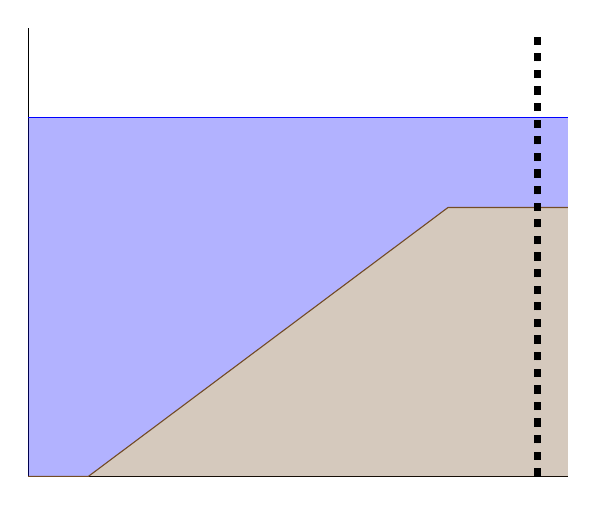
\begin{tikzpicture}
	\begin{axis}[ 
	axis y line*=left,
	axis x line*=bottom, 
	xtick={-0.1},  
	ytick = {-0.1}, 
	xmin=5, 
	xmax=14, 
	ymin =0, 
	ymax = 0.5]
	
	\addplot [name path=b,brown!60!black] coordinates {(5,0) (6,0) (12,0.3) (14,0.3)};
	
	\path[name path=axis] (axis cs:5,0) -- (axis cs:14,0);
	
	\addplot [name path=a,blue] coordinates {(5,0.4) (14,0.4)};
	
		\addplot [
		thick,
		color=brown!60!black,
		fill=brown!60!black, 
		fill opacity=0.3
		] fill between[of=b and axis];
		
	\addplot [
	thick,
	color=blue,
	fill=blue, 
	fill opacity=0.3
	] fill between[of=a and b];
	
	
	%\addplot [black,dashed,thick] coordinates {(5.7,0) (5.7,0.5)};
	
	%\addplot [black,dashed,thick] coordinates {(10.5,0.23) (10.5,0.5)};
	
	%\addplot [black,dashed,thick] coordinates {(12.5,0.3) (12.5,0.5)};
	\addplot [black,dashed,thick] coordinates {(13.46,0) (13.46,0.5)};
	\addplot [black,dashed,thick] coordinates {(13.48,0) (13.48,0.5)};
	\addplot [black,dashed,thick] coordinates {(13.5,0) (13.5,0.5)};
	\addplot [black,dashed,thick] coordinates {(13.52,0) (13.52,0.5)};
	\addplot [black,dashed,thick] coordinates {(13.54,0) (13.54,0.5)};
	\end{axis} 
	
	
	
	\end{tikzpicture}
\end{document}